\documentclass[12pt]{ociamthesis}  % default square  
%\documentclass[12pt,beltcrest]{ociamthesis} % use old belt crest logo
%\documentclass[12pt,shieldcrest]{ociamthesis} % use older shield crest logo

%load any additional packages
\usepackage{amssymb}
\usepackage{amsmath}
\usepackage{algorithm}% http://ctan.org/pkg/algorithms
\usepackage{algpseudocode}% http://ctan.org/pkg/algorithmicx
\newcommand{\var}[1]{{\ttfamily#1}}% variable
\usepackage{graphicx}
\usepackage{pgfplots}
\usepackage{filecontents}
\usepackage{tikz}
\usepackage{color}
\usepackage[bottom]{footmisc}
\usepackage[T1]{fontenc}
\usepackage[utf8]{inputenc}
\usepackage{tabularx,ragged2e,booktabs,caption}
\newcolumntype{C}[1]{>{\Centering}m{#1}}
\renewcommand\tabularxcolumn[1]{C{#1}}
\usepackage{hyperref}
\usepackage{rotating}
\restylefloat{table}
\usepackage{longtable}
\usepackage{lscape}
\tikzstyle{startstop} = [rectangle, rounded corners, minimum width=3cm, minimum height=3cm,text centered, draw=black, fill=blue!30]
\tikzstyle{arrow} = [thick,->,>=stealth]

%input macros (i.e. write your own macros file called mymacros.tex 
%and uncomment the next line)
%\include{mymacros}

\title{Predicting Trust for\\[1ex]     %your thesis title,
        Online Social Media}   %note \\[1ex] is a line break in the title

\author{Kaushalya Kularatnam}  %your name
\college{Wolfson College}  %your college

\renewcommand{\submittedtext}{Dissertation submitted for the degree of}
\degree{Master of Science in Computer Science}     %the degree
\degreedate{September 2014}         %the degree date

%end the preamble and start the document
\begin{document}

%this baselineskip gives sufficient line spacing for an examiner to easily
%markup the thesis with comments
\baselineskip=18pt plus1pt

%set the number of sectioning levels that get number and appear in the contents
\setcounter{secnumdepth}{3}
\setcounter{tocdepth}{3}


\maketitle            % create a title page from the preamble info

\begin{abstract}

The proliferation of Internet usage has resulted in huge amounts of information being made available online. We instinctively trust our closest friends or relatives, or information presented to us by people in our networks[2]. The fact that there is so much information, often with rumours or inconsistencies makes it hard to know who or which information source to trust, or much worse makes it hard to not trust information that we believe come from a reliable source.\\*\\*
This thesis looks at identifying trust metrics for online social media, particularly in the case of Twitter. We look at the characteristics of trustworthy and untrustworthy tweets for example the length of tweet, the amount of retweets, followers etc and learn patterns from this to create a model which determines if a tweet is trustworthy or not.
We compare the results obtained from two different models, based on two machine learning techniques.

\end{abstract}            % include the abstract
\begin{acknowledgements}
I would like to express my sincere gratitude to Dr.Jason R. C. Nurse for his untiring patience, direction and guidance throughout this project.\\*\\*
I would also like to thank Professor Michael Goldsmith and Dr.Ioannis Agrafiotis for their advice and input. \\*\\*
Finally I thank my friends, sister and parents for their support and encouragement throughout this course. 
\end{acknowledgements}   % include an acknowledgements.tex file
\begin{romanpages}          % start roman page numbering
\tableofcontents            % generate and include a table of contents
\listoffigures              % generate and include a list of figures
\end{romanpages}            % end roman page numbering

%now include the files of latex for each of the chapters etc
\part{Background}
\chapter{Introduction}
In this chapter we introduce this research report on the topic of information trust metrics in social media. We begin with the motivation behind the research and the general aim of the project. This is followed by the specific goals that we intend to achieve by the end of this research. Finally we give an overview of how this document is structured. 
\section{Motivation}
Online interactions represent a complex blend of human actors and technological systems\cite{2}. In recent years, the type of content available on the Web has transformed greatly and the interactions online between individuals has become increasingly popular\cite{5}. A big contributor to this is social media networks such as Facebook, Twitter and Google Plus and Question and Answer platforms like Yahoo Answers, Quora and Stackoverflow. The general content that is made available to us by fellow users through this medium of information propagation could range anywhere from opinions, facts, reviews and criticism to real and fake photos, videos, animations etc.\\*\\*
Although an abundance of freely shared and communicated content is advantageous for official (e.g, crisis response\cite{25}, government announcements \cite{26}), commercial (e.g, interactions with customer base) and social reasons (e.g, event planning, dating) significant concerns have been raised about the quality, provenance and trustworthiness of this content \cite{13,27,28}. Furthermore in several cases it is also not possible to make an informed judgement on the trustworthiness of a person, account or entity online. Verified Twitter\footnote{https://support.twitter.com/articles/119135-faqs-about-verified-accounts} and Facebook\footnote{https://www.facebook.com/help/196050490547892} profiles go some way to ensure that the identity of an entity is verified independently therefore validating the authenticity and to some extent the content of that entity. These verifications, however are only intended to confirm identity and do not necessarily always relate to the quality of the individuals content. We should also note that hacks of social media accounts render such `verifications' as useless and fairly damaging (e.g, AP Twitter hack causing panic on Wall Street sending the Dow Jones industrial average plummeting to a 143-point fall \cite{16}).\\*\\*
It is impossible for us as human beings to manually verify every piece of information presented to us as a result of the sheer volume of content online. To automate the task of trustworthiness assessment several researchers have proposed metrics, but developments in this field are still ongoing. The metrics are based on factors which are believed to influence trustworthiness. Example factors include quality, trust, provenance \cite{13}. Research by Meredith et al. (2012)\cite{17} also details some Twitter-based features and provides the credibility impact ratings (How these factors impact the credibility of the tweet). This project aims to progress the idea of automated assessment further and propose a new approach to the problem. 
\section{Aims and Approach}
The broad aim of this work is to explore the provisions of a systematic approach for assessing information on the Internet, with the specific test case of Twitter. There has been a significant amount of research conducted in this area, which we will detail in the next section. Our approach aims to be different in the way that we identify trustworthy information and sources. That is, in our work we aim to use the features and other characteristics of news agency tweets to infer what trustworthy posts resemble on Twitter. Our assumption uses features of news profiles and fake profiles to infer what trustworthy and untrustworthy Twitter pages look like. We then seek to use this knowledge to train a supervised Machine Learning model that can later be applied to predict the trustworthiness of newly acquired tweets, and evaluate the accuracy of our model. This project will aim to improve upon current research and explore an alternative solution to help people, official organisations and groups to identify trustworthy content.  
\section{Objectives}
As mentioned in the section prior this project explores the problem of analysing the trustworthiness of information on the Twitter social media platform. We focus on the following objectives to achieve our stated research aim: \\*\\*
1. Identify the factors that affect trustworthiness in online social media and narrow it down to the factors that could be important in the case of Twitter. \\*\\*
2. Gather relevant data from Twitter such that we have a wide range of trustworthy and untrustworthy tweets for training and analysis using our supervised Machine Learning application.\\*\\*
3. Implement three Machine Learning\footnote{Field of study that gives computers the ability to learn without being explicitly programmed\cite{18}} models. We pass the features gathered from the tweets to the model and tweak the features, derive new and relevant features from that gathered such that the accuracy of the model reaches 80\% or more. \\*\\*
4. Compare the different machine learning models we have chosen, in terms of accuracy and efficiency and pick the model that best suits our problem. \\*\\*
5. Evaluate the accuracy of the chosen Machine Learning model by providing it with new test data(which is completely independent from our training and test sets) for trustworthiness prediction. 
\section{Thesis Structure}
$\textbf{Chapter 2}$ Provides background into existing research and engages in a critical review of the literature. \\*\\*
$\textbf{Chapter 3}$ This chapter details our understanding and approach to the problem and our proposed solutions. \\*\\*
$\textbf{Chapter 4}$ We discuss the data collection and classification methodology as well as an explanation behind the chosen Features for our models. \\*\\*
$\textbf{Chapter 5}$ We explain the theory behind the Machine Learning algorithms used in our development. Namely, Logistic Regression, Support Vector Machines and Random Forests.  \\*\\*
$\textbf{Chapter 6}$ In this chapter we provide details on the testing and results of our models along with some discussion on the methods used in our experiment. \\*\\*
$\textbf{Chapter 7}$ We finally conclude by reflecting on our approach, experiment and results as well as a discussion on future work and improvements.  \\*\\*


\chapter{Literature Review}
Our work draws on a significant amount of previous research. In this chapter, we will critically reflect on and discuss that work and its impact on the social media research field.
\section{Information Trustworthiness Online}
In this section we discuss the state-of-the-art in this field and seek to understand what information trustworthiness is online. Information Trustworthiness, in the context of online interactions is content that is reliable and credible. Trustworthiness online could be assessed by any combination of factors including User-based Features, Message-based features, Topic-Based features and Propagation-Based features\cite{12}. Our goal here is to identify the different types of factors and features explored and their impact on trustworthiness, and narrow it down to what would be most relevant for our particular case, i.e, Twitter. In this document, by trust $\mathbf{Factors}$ we mean factors such as Corroboration, Competence of the Source, Propagation, Information Provenance etc. Trust \textbf{Features} would be domain specific and closely related to the problem. For example, the number of likes of a Facebook page, or the number of friends of a Facebook user would all be referred to as features.
\subsection{Non-Twitter Based Research} 
A paper by Yahoo! Research\cite{5}, addresses the problem of finding high quality content in community-driven question/answering sites. Quality of content might not always correlate with its trustworthiness. Research and Literature though, has highlighted that they certainly share similar characteristics. For this research, they looked specifically at Intrinsic content quality (Punctuation, typos, syntactics and semantic complexity, grammaticality), User Relationships (User \textit{a} answered a question by user \textit{b}) and Usage statistics (number of clicks on a question). One of the primary differences of this research to our problem is that the actors involved are different. In the question and answer domain, there is an asker, answerer and an evaluator\footnote{People who up vote answers, like answers, modify them or question them}. In the case of Twitter there is only a User and a `Fan'. We use the word fan to describe any other Twitter user who has favourited or retweeted the tweet. In terms of the domain, question and answer platforms are used by users looking for help with a particular situation\cite{5}, however broadcasting platforms such as Twitter are used as ways of displaying ones thoughts, current events or generally making one's voice heard. ``Size Matters" by Blumenstock\cite{4} proposes word count as a factor for determining article quality. While this might stand true for articles on Wikipedia, the platform on which they base their research, this may not necessarily make a huge difference in the results we get since a tweet is a maximum of 140 characters regardless. Smyth et al. \cite{10} state that features such as regularity with which bloggers post, timeliness of the posts, post length, spelling quality and appropriate use of capitalisation and emoticons in the text link to an article's credibility, a factor which has close links to Trustworthiness. They specifically look at Amazon Reviews and TripAdvisor for their test cases.  In Nurse et a. \cite{7}, they identify timeliness as one of the main factors in trustworthiness. While this may be true in crisis situations or in relation to current affairs, this may not necessarily apply to general tweets, or tweets about past events. They also state that information completeness, complexity and relevance are important factors in assessing trustworthiness. Besides they've identified a fair few factors such as authority/reputation affecting trustworthiness, which we have factored into our model. Goldsmith et al.\cite{13} provides a state of the art review of the current work and considers the links between provenance, quality and trustworthiness. They provide a number of factors which undoubtedly would have an influence on our analysis.
\subsection{Twitter Based Research}
Gupta et al. \cite{11} is quite closely related to our research. However, the address tweets of high impact events as opposed to any general tweet. In it they identify no. of characters, emoticons present in a tweet, number of followers, length of username and use of pronouns and swear words as some of the more important content-based credibility features. Carlos et al. \cite{12} look at analysing microblog postings from trending topics and aim to classify them as credible or not credible. They categorise factors into four different sections. They are Message-based, User-based, Topic-based and Propagation-based factors. They identify a range of features, such as length of words, length of characters, contains a question mark, distinct hashtags etc. Morris et al. \cite{17}, examine key elements of the information interface for their impact on humans' credibility judgements. They show that users had difficulty determining the truthfulness of content and that their judgements were based on heuristics such as retweets and topic-related user names were considered more trustworthy than another. For example, the user name `TechCrunch' for a Twitter profile would appear more trustful to humans than a name such as `Jo' if they were to believe news about technology. Researchers at the University of Washington \cite{43}, are currently working on looking at the relationship between various web links within tweets, and the quality of information spread during the Boston marathon bombing incident\footnote{\url{http://en.wikipedia.org/wiki/Boston_Marathon_bombings}}. They are hoping to develop a tool, which would let users know when a tweet is being questioned or proven untrue by another tweet. \\*\\*
We discussed the different types of research both Twitter based and non-Twitter based conducted in this domain, in the above section. The following section will detail and explain some of the metrics, models and methodologies used in the past to predict quality, credibility or trustworthiness of tweets. 
\section{Measuring Trustworthiness}
\subsection{Metrics and Models}
Here we focus on the types of features/characteristics that researchers have chosen in the data to analyse, as well as the techniques that have been used.
Nurse et al. \cite{7}, reflects on information trust and quality metrics. They propose some new metrics that are worthy of consideration. This acted as a good source to think about different metrics for trust on social media and build our research.
In our research we are not necessarily looking at content quality hence we do not have these characteristics factored into our model. In the Yahoo! research\cite{5}, they selected the 20 most significant features for question quality using a chi-squared test and discovered that the precision and recall improved slightly if they used the top 10 features as opposed to all the features. The precision, recall and Area under curve\footnote{A graph of True positives Vs False positives. See Chapter 6 for explanations} for finding high quality answers was nearly 90\% in comparison to the 70\% obtained for question quality. This probably could be due to the fact that they used the the text as a baseline and the answer text would have more content to it than the question hence a more accurate prediction in the latter case. \\*\\*For the experimentation in \cite{7} they used the following factors as basis : Corroboration (extent to which the same information originates from different sources), Social-Jargon (e.g Emoticons, Shouting), Competence of the Source (Level of expertise of the source of information), Location of the source. In ``Information Credibility on Twitter"\cite{12} they used Machine Learning techniques such as the Support Vector Machines (see 5.3), decision trees (see 5.4.1), decision rules and Bayes networks but achieved best results using a J48 decision tree method. \\*\\*
The article about Wikipedia \cite{4}, which states how word count affects quality, achieved above a 95\% accuracy on Machine Learning models such as multi-layer perceptron, k-nearest neighbour classifier, a logit model and a random forest classifier. Kumaraguru et al. \cite{11}, state that they found that on average 30\% content about an event provides situational awareness information and 14\% was spam. They also found that only 17\% of the situational awareness information was credible\cite{11},. They mention that one of the drawbacks and limitations with their data collection method was that they had to allow human annotators to annotate the classifications and would like a more automated system to establish ground truth. Our proposed algorithm seeks to tackle this problem by learning from known Trustworthy and Untrustworthy. 
\subsection{Data Collection and Classification Methodology}
We discuss how different researchers approach the problem of classifying data into different classes. Our approach to classification for this problem was exploring news agency tweets as annotated Trustworthy content and fake/known parody accounts as Untrustworthy content. However it is interesting to see how other researchers have handled the data classification problem so we detail some classification methods in this section. The dataset used by Yahoo! Research consisted of 8,366 questions/answer pairs and 6665 questions. There were independent human editors who labelled all of the above data for quality. One would find that a drawback with such a method for labelling data could be that it might be slightly biased based the ranker's knowledge / previous experience with the topic at hand. TThe paper ``Tweeting is Believing"\cite{17} states that they find that users are poor judges of truthfulness based on content alone. Our approach tries to be different as we do not involve human annotators at the Classification stage, although we appreciate that it is an assumption that all news tweets are Trustworthy. For the study on Amazon and TripAdvisor they collected four large review datasets and they relied on the response provided by the user in whether they found the reviews to be helpful or not to establish ground truth. In the paper about credibility of tweets \cite{11} they use the Twitter Streaming API to search for keywords and select tweets based on that. They also used the Trends API which returned the trending current trending topics in Twitter. Human annotators were used to rate the credibility of the tweets into four different categories such as Definitely Credible, Seems Credible, Definitely Not Credible, I cannot Decide. The paper by Castillo \cite{12} looks at time sensitive information such as current news events and hence they used the Twitter Monitor\footnote{http://twittermonitor.net} which monitors sharp increases in the frequency in a set of keywords in a tweets. For classifying they used the Mechanical Turk\footnote{http://www.mturk.com} which involved asking evaluators to assist them with classification. 
\section{Summary}
This review enabled us to understand factors and features, metrics and models and how they are all connected to each other. We also learned about the ongoing research in this field in both academia and in the industry. We realise that the problem of determining Trustworthiness of content still exists and we were able to identify three key areas in terms of factor selection that we would focus our research on.  We chose Message content-based factors, User-based factors and Tweet-based factors, the reasons behind this selection will be explained in future chapters. The next chapter explains in detail our approach to the problem and how we compartmentalised the  necessary steps to take to achieve our aim.  





\part{Model Theory}
\chapter{Logistic Regression}

\section{Background }

{In the early 19th Century[1], Probit Analysis was widely used in academia and in the Industry. As time went by, the Probit Model which is closely related to the Logit Model became less popular and the latter gained popularity. The Logit Model forms the basis of Logistic Regression. Logistic Regression is a widely used and important Linear Machine Learning model. By Linear we mean we take inputs and compute a signal that is a linear combination of the inputs with weights. Although poorly named Logistic Regression, it is essentially a probabilistic classification algorithm and it builds the foundation for more complex methods like Neural networks. Logistic Regression can be used for binary classification and can be extended to multi class classification, however we will specifically look at the algorithm for binary classification since our problem is binary. In the next few pages we will look at how our algorithm works and the underlying logic behind it.}

\section{Derivation}
$\mathbf{Problem}$ : Trust Worthiness of tweets posted on Twitter.\\*
$\mathbf{Structure}$ : Our data is a collection of $x$ and $y$ data points where $x_i$ is a $d$ dimensional vector and $y$ is a True or False classification\\*
\centerline{$D = ((x_1,y_1),..,(x_n,y_n)) , x_i \in \mathbb{R}^d$  and  $y_i \in {0,1}$}
$\mathbf{Input}$ : $x_1$ = FrequencyOfTweets, $x_2$ = FavouriteCount, $x_3$ = RetweetCount, $x_4$ = InReplyToStatusID, $x_5$ = InReplyToUserID, $x_6$ = Hashtags, $x_7$ = UserMentionID, $x_8$ = URL, $x_9$ = MediaURL, $x_{10}$ = MediaType, $x_{11}$ = PossiblySensitive, $x_{12}$ = Language, $x_{13}$ = TweetLength , $x_{14}$ = Location, $x_{15}$ = Description $x_{16}$ = UserAccountURL, $x_{17}$ = Protected, $x_{18}$ = FollowersCount, $x_{19}$ = FriendsCount, $x_{20}$ = ListedCount, $x_{21}$ = FavouritesCount, $x_{22}$ = Verified, $x_{23}$ = GeoEnabled, $x_{24}$ = StatusesCount, $x_{25}$ = ProfileBackgroundImageURL, $x_{26}$ = ProfileUseBackgroundImage, $x_{27}$ = DefaultProfile, $x_{28}$ = IsItARetweet\\*\\*
$\mathbf{Model}$ :  Logistic Regression is a discriminative model and we want to model the probability of the information being trustworthy, given some data about the tweets. We write $y_i$ as a Bernouli Random variable with probability $\sigma(w^Tx_i)$ where each of the $y_i$'s are independent. The $w$ here is the parameter and the $x_i$ are fixed and non random. We give weights to each of the variables to get a linear combination. \\*
\centerline{$w_0 + w_1x_1 + w_2x_2 + ... + w_ix_i = w^TX$ where $X = (1,x_1,x_2,x_3)$} \\*
Here the coefficient W tells us something about how the individual variables are affecting the probability. For instance if W is negative then the probability decreases when the variable increases in value and vice versa. The coefficients also tell us which variables are more influential than the others. A large coefficient regardless of whether it's positive or negative influences the decision more thanks a small coefficient. \\*

Let us say that the probability of the the tweet being trustworthy is $P$. Then the probability of the tweet not being trustworthy is $1-P$.

The odds ratio then is : P / 1 - P 
We now take the natural logarithm of this : ln (P / 1-P)
ln (P / 1 - P ) = $w^Tx$
Now if we take the exponent on both sides we get 
P / 1 - P = $e^{w^Tx}$
P = (1 - P)*$e^{w^Tx}$
P = $e^{w^Tx}$ - P*$e^{w^Tx}$
P + P*$e^{w^Tx}$ = $e^{w^Tx}$
P(1 + $e^{w^Tx}$) = $e^{w^Tx}$
P = $e^{w^Tx}$ / (1 + $e^{w^Tx}$)
In this equation on the R.H.S if $e^{w^Tx}$ tends to +infinity numerator in the formula below will be very huge and so will the denominator and the ratio will be close to 1. If $e^{w^Tx}$ tends to -infinity both numerator and denominator would be very small and be close to 0. If $e^{w^Tx}$ is 0 then $\sigma(e^{w^Tx})$ = 1/2. 
Multiplying the R.H.S by  $e^{-w^Tx}$ we get 
P = 1 / 1 + $e^{w^Tx}$

(Draw a sigmoid function in 28). 

$0 <= \sigma(e^{w^Tx}) <= 1$
Logistic Function : $\sigma(w^Tx) = 1 / 1 + e-w^Tx$\\*

The Target Function f : $R^d$ -> [0,1]
$P(y|x) = \{f(x) for y=+1, 1 - f(x) for y=-1\}$	\\*

Our final hypothesis which we call h(x) is what we need to learn, which has the form of logistic regression,  and we would claim that this is approximately equal to f(x). So we basically get the weights, multiply it with x and pass it through the non-linearity and make sure that it reflects f(x) as closely as possible. Our aim is to make this as close as possible, and what we can change here is our parameter which is W. So in other words, we know f(x), we chose Ws to give us h(x) which closely resembles f(x). 

$h(x) = \sigma(wTx) =approx f(x)$\\*

$\mathbf{Maximum Likelihood Estimate}$[14] : Given below is how we compute the Maximum likelihood estimation for the Logistic Regression Model, for our binary scenario.\\*
W = Parameter \\*
D = Data\\*
$W_{MLE}$ = Maximum Likelihood estimate for our parameter w\\*
$P(D|w)$ = Probability of the Data given w\\*
$P(y|x)$ = Probability of y given x

$W_{MLE}$ $\in argmax$  $P(D|w)$\\*

$P(D|w)$ = $\prod_i=1^n P(y_i|x_i,w)$ \\*
We can write the probability mass function of a bernouli as : 
= $\prod_i=1^n \sigma(w^Tx)^{y_i}(1-w^Tx)^(1-y_i)$
To get the Maximum likelihood estimate we would want to maximise P(D|w). We can now take the log of P(D|w) and maximise this or minimise - log P(D|w). 
L(w) = - log P(D|w) = - sum i=1 to n $y_i$ log $W^Tx$ + (1-$y_i$)log(1-$W^Tx$)
We need to take the gradient with respect to W of sum i=1 to n $y_i$ log $W^Tx_i$ + (1-$y_i$)log(1-$W^Tx_i$). 
derivative log sigma(W^Tx) 




A brief comparison of Logistic Regression with some other classification models are given below : 

Linear classification: 

We take our hypothesis to be a decision, and this decision (+/- 1) is a direct result of signal. In the following diagram our inputs are x1?xd where X(dash on top) is a d dimensional vector and we sum it and pass it through the following threshold to get a decision. Insert Diag 1 

Linear Regression 

In the case of Linear Regression we do nothing to the signal. Here we output what we input, the input being the sum of vectors x1..xd. Insert Diag 1

Logistic Regression 

In Logistic regression we will take our sum and apply a non-linearity to it. Here theta the logistic function is not as harsh as the Linear Classification and the output would be interpreted as a probability. Again in our diagram we have a d dimensional vector x and the sum is passed through this function to give us a probability.  insert Diag 1


Pros : 

1.Small number of parameters : In the above the number of parameters would be (d+1). What this means is that even if the dimensions increase, the number of parameters only linearly increases. 
2.This model is Computationally efficient to estimate the w parameter. We use Newtons method  
      which is a very efficient second order method which is guaranteed to converge to a Maximum    Likelihood estimate. 
3. You can extend it to multi class classification
4. Forms the foundation for some of the more complex methods like neural networks.

Cons : 
Performance is not necessarily as good as some of the best performing methods such as random forests, boosted methods and support vector machines. This however, greatly depends on the nature of the problem and from what we can see this has performed quite well for our problem. 

Foot Note : 1The MLE proof stems from some notes from reference[14]
\chapter{Data Collection and Feature Selection}
\section{Data Collection}
\subsection{Training and Testing}
Data retrieval for this project was from the twitter API which is located at \url{https://dev.twitter.com}.  Twitter has many APIs, each API representing a facet of twitter. They are Twitter for websites, Search API, REST API and Streaming API. The Twitter REST API was used for this specific task.\\*\\*
Initially you are required to set up an account and a password after which you will receive an AccessToken, AccessSecret, ConsumerKey and ConsumerSecret which would then be needed to authenticate you to use the API. You make restful calls using the above credentials. The call
`GET statuses/user\_timeline' returns a collection of tweets posted by the user, who is identified by the user ID or screen name parameters provided. If the account is protected, you may receive tweets only if your user account has been approved by the user or if you are the user himself. 
For example the following call would retrieve the last 200 tweets by the Twitter User named BreakingNews. Various different parameter combinations can be set to retrieve a subset of the necessary data. 
\url{https://api.twitter.com/1.1/statuses/user\_timeline.json?screen\_name=BreakingNews&include_entities=true&include_rts=true&count=200}
The above call gives us only the tweets by the user, and doesn't necessarily give us a lot of information on the user itself. For this we look up the user details with the following request.  
\url{https://api.twitter.com/1.1/users/lookup.json?screen\_name=Independent}
This would give us the User Information of the user who's screen name is the Independent. 
Once data is received this way, we store the last ID for each user in the dataset, such that we then make the next call using the last ID. The data is received in JSON Format, which is then slightly modified to fit our needs and then converted to CSV format to pass on to our Machine Learning algorithm. 
We used twenty widely popular News Websites such as the Guardian, BBC, CNN etc and found around twenty five fake accounts to retrieve untrustworthy data. We have a dataset with about 20,000 tweets, collected over 5 days. The above code was written in java and Manipulation of the received raw data was done using the north concepts library which handles data conversion, processing and transformation in java applications. 
\subsection{Prediction}
The above data collection method relates to how we gathered data for the Initial stage of our analysis, that is training and testing. This sub section deals with our data collection methodology for our verification stage. We collection 39 individual tweets from very different users. Of this we had 20 Untrustworthy tweets and 19 Trustworthy tweets. When choosing untrustworthy tweets, we referred to news paper articles which point out some of the rumours that were spread during crisis situations around the world. We hand picked some of the highlighted tweets in these articles. When choosing Trustworthy tweets for our analysis we looked at further news agency profiles which we hadn't used in our training. Since we were selecting tweets, we had to retrieve the features of these tweets using the tweet ID of the tweet, which is found at the top of the URL of the tweet detail page. For example, in this URL, \url{https://twitter.com/ObamaNews/status/506469766815416320} the latter part gives us the ID of this specific tweet. We use this ID in a restful call as follow : \url{https://api.twitter.com/1.1/statuses/lookup.json?id=506469766815416320}. Once we receive the features of the necessary tweets, the processing of the tweets and filtering is similar to how we processed our training data. 
\newpage
\section{Feature Selection} 
The raw JSON that we receive from the REST calls have a huge amount of information that we may not need. Some of the features retrieved have a significant amount of null values which might cause problems in our analysis later. For this reason some features of the returned results were dropped at various stages in the program. (Some at initial data collection level and some later on in the actual dataset used for measure).
We categorised the features that we would use for our training into three different types of sections. They are : \\*\\*
$\textbf{Tweet Based Features : }$ This feature set primarily dealt with features pertaining to the Tweet in question. Examples of some of the tweet based features used in our model are - In reply to a status or a user, Number of retweets, number of times the tweet has been favourited and the number of hashtags in the tweet.  \\*\\*
$\textbf{User Related Features : }$ This feature set handles features that relate to the user.  Verified Profile, Number of Statuses published, Does profile use a background image and Number of followers are some examples of user related features that we used in our model. \\*\\*
$\textbf{Message Content Based Features : }$ This feature set is a collection of features which are mostly derived from the message content and other attributes, which deal with the actual contents of the tweet. Length of the tweet, Emotions in the tweet and Keywords used are some of the features that we included the analyse message content.\\*\\*
The complete list of features retrieved and used are given in the next section. \\*
\section{Features}
The following table explains the features in detail and the reasoning behind the inclusion or exclusion of this information in our classifiers. 
\newpage
\begin{landscape}
\centering
\begin{longtable}{|C{1.00in}|C{2.50in}|C{.60in}|C{5.00in}|}
\caption{Tweet Based Features} \\
\toprule[1.5pt]
Feature Name & Explanation & Included & Reason \\\midrule
Created\_At & UTC time for when this tweet was created & Yes & This could be used to see if frequency has an impact on trustworthiness. For instance if the number of tweets per minute posted by the user has an impact on the trustworthiness of a user. \\
\hline
Id & Tweet ID & No  & The ID of the tweet could in no way impact our analysis \\                                                                                                                                                                                                                            
\hline
Id\_str & Tweet ID in String Form & No  & As above \\                                                                                                                                                                                                                                                                            
\hline
Text & Actual Tweet  & No  & We have used the text of the tweet to analyse the contents of the message. These features will be explained in depth in the table on Message Based Features. \\
\hline
Source & This is the Utility used to post the tweet, as an HTML-formatted string & No  & Although it would be interesting to see if there is any correlation between the utility used to post the tweet and the trustworthiness of the tweet, most tweets are posted from the twitter web client which has a source value of `web' hence this would not make a huge difference. \\ 
\hline
truncated & If the tweet was truncated or if it is the original length & No  & The Twitter API says that this feature is rarely ever used since twitter now rejects long tweets as opposed to truncate them - we saw no reason to use this. \\
 \hline
In reply to Status id & If this tweet was a response to a status then the integer representation of the ID of the status replied to & Yes & This feature would tell us if it is a tweet or a reply to a tweet, hence we used this.\\
\hline
In reply to Status id str & If this tweet was a response to a status then the string representation of the ID of the status  & No  & This is just a repetition of the previous feature in String Form\\
\hline
In reply to user id & If this tweet was a response / message to a user, the integer representation of the UserID & Yes & This feature can be used to check to see if it is a response to a user or a tweet. \\
\hline
In reply to user id str & If this tweet was a response / message to a user, the string representation of the UserID  & No  & Repetition of previous information above. \\     
\hline                                                                                                             
In reply to screen name & If the tweet is a response then this field will have the screen name of the original author  & No  & Repetition of previous information above.  \\    
\hline                                                                                                                                                                                                          
user  & This is an embedded JSON array containing information about the user who posted the tweet. This list contains only basic user information. & No  & Since we made another request with the actual user ID to retrieve information about the user this array will just be a replica of what we already have. The advice from Twtitter API is also such that embedded information such as this are unreliable. \\
\hline
geo & Deprecated   & No  & Although this appears as part of the JSON received this feature is deprecated in this API. \\
\hline
coordinates  & The geographical location of the tweet if provided. & No  & In almost all the data we received this information is not present hence we decided to drop it. However user locations are available on the user profile. \\
\hline
place  & If a value is present then this shows that the tweet is associated but not necessarily originating from this place. & No  & Again a huge majority of the samples we received didn?t have this information so we decided to not include this information. \\
\hline
contributors & A collection of brief user objects showing the people who contributed to the authorship of the tweet. & No  & This will only work if the user has turned the contributors enabled feature on. This is a beta feature and is not available to all the users at this point of time, hence we decided to not include this in our analysis. \\
\hline
Retweet count  & Number of times a story has been retweeted & Yes & This could be an important indication of propagation of data and how information spreads hence we included this in our model. \\
\hline
Favourite count & Number of times a story has been favourited & Yes & The times a story has been favourited may also play an important role on trustworthiness, therefore this is included.\\
\hline
entities & Entities provide information about the text of the tweet without having to parse the text to find out the structure. It shows you URLs, MediaURLs, Hashtags and symbols used in a tweet. & Yes & This information is deemed valuable as we can analyse the differences in structure of a trustworthy tweet with an untrustworthy one. e.g : Analysis such as do trustworthy tweets always come with a URL, or Image accompanying the story etc.\\
\hline
favourited & This indicates if the tweet has been favourited by me (Authenticating User) & No  & This piece of information is irrelevant, since it concerns the authenticating user (me in this instance) hence the exclusion.  \\
\hline
retweeted & This indicates if the tweet has been retweeted by the authenticating user.  & No  & This piece of information is irrelevant, since it concerns the authenticating user (me in this instance) hence the exclusion. \\
\hline
Possibly sensitive & This field only comes up if the tweet contains a link. This is an indicator, that the URL in the tweet may contain media that may be sensitive. & Yes & A value in this field indicates two things : That a URL is present and if the URL is sensitive or not. Hence this feature could be useful for our analysis. \\
\hline
lang  & This indicates a BCP 47\footnote{\url{http://tools.ietf.org/html/bcp47}} language identifier which shows the language that was detected by the machine for the tweet. & Yes & This feature is used - since we want only tweets that are in english \\
\hline
frequency  & DERIVED : This is a derived value from the Messages received. We Take the first and Last tweets of a User Over a time period and calculate the frequency of the tweets  & Yes & This could be an important indicator in informing us patterns for different types of users, hence we use this feature.\\
\hline
Is It A Retweet & DERIVED : This is a column that checks if the tweet is a retweet or an original & Yes & This could be used to weed out duplicates.\\  
\hline                                                                                                                                                                                                            
\bottomrule[1.25pt]
\end{longtable}
\label{tab:LPer}
\end{landscape}

\begin{landscape}
\centering
\begin{longtable}{|C{1.00in}|C{2.50in}|C{.60in}|C{5.00in}|}
\caption{User Related Features} \\
\toprule[1.5pt]
Feature Name  & Explanation & Included In & Reason  \\\midrule
Id   & Unique Identifier for User                                                                                                     & No          & Not very useful for analysis                                                                                                                                                                     \\
\hline    
Id str & String representation of the id above                                                                                          & No          & Not very useful for analysis                                                                                                                                                                     \\
\hline    
Name & The name of the user as they?ve defined it                                                                                     & No          & Not very useful for analysis                                                                                                                                                                     \\
\hline    
Screen Name  & The name a user is identified with on twitter                                                                                  & No          & This feature could have been used at some point to weed out badly spelt or written screen names but we have not used it in this iteration.                                                       \\
\hline    
Location  & The user defined location for this account.                                                                                    & No          & Including this diluted our analysis since we had profiles from all over the world, and we only had 40 profiles in total.                                                                         \\
\hline    
Description & A string describing the users account                                                                                          & Yes         & The description itself is not used in our analysis however the length of the description string is used in our analysis.                                                                         \\
\hline    
URL  & A URL associated with the user provided by him/her                                                                             & Yes         & We check if the user has a URL or not. We do not use the URL itself.                                                                                                                              \\
\hline    
Entities  & Entities that have been parsed from the URL or description fields.                                                             & No          & This information has already been taken into account from other features.                                                                                                                        \\
\hline    
Protected & This indicates if the user has chosen to protect their tweets                                                                  & Yes         & This might have some significance as well hence included.                                                                                                                                        \\
\hline    
Followers Count  & The Number of followers this User / Account currently has                                                                      & Yes         & This is a very important feature, hence it is included in both our classifiers.                                                                                                                  \\
\hline    
Friends Count & The Number of users this user follows on twitter                                                                               & Yes         & This is also a very important feature hence it is included.                                                                                                                                      \\
\hline    
Listed Count                       & This is the number of public lists this account is a member of.                                                                & Yes         & This is also a very important feature hence it is included.                                                                                                                                      \\
\hline    
Created At                         & The date and time this account was created                                                                                     & Yes         & This feature also might be an indicator of the trustworthiness of the source/ account.                                                                                                           \\
\hline    
Favourites Count                   & The amount of tweets this user has favourited from the date of opening the account                                             & Yes         & It will be interesting to see if there are any patterns in how active the user is in terms of favouriting other tweets and responding.                                                           \\
\hline    
UTC Offset                         & This is the offset from GMT given in seconds.                                                                                  & No          & This is not used since Location has already been used once.                                                                                                                                      \\
\hline    
Time Zone                          & This string gives the time zone within which the user profile is within                                                        & No          & Once again this feature would be a duplicate of Location hence we did not use it.                                                                                                                \\
\hline    
Geo Enabled                        & If true this means that the user has enabled geo tagging for his tweets.                                                       & Yes         & Again, it would be interesting to identify any patterns amongst the different types of users.                                                                                                    \\
\hline    
Verified                           & Verified Twitter accounts are accounts which Twitter has verified - stating that the user is who they say they are on twitter. & Yes         & This could be a very important factor in predicting trustworthiness hence it is included in our model.                                                                                           \\
\hline    
Statuses Count                     & The number of tweets published by the user.                                                                                    & Yes         & It would be interesting to see the correlation or between the total number of statuses and Trustworthiness factor.                                                                               \\
\hline    
Lang                               & The BCP 47 code for the language used by the user. This is self declared.  & No          & This feature is not used since it could negatively impact the analysis, or create a bias that is unnecessary.                                                                                    \\
\hline    
Status                             & This gives information about the users most recent tweet.                                                                      & No          & We will not be using this feature since we have all the necessary information we need about the users tweets from our primary request to the API.                                                \\
\hline    
Contributors Enabled               & This allows the tweets by this account to be coauthored by another account                                                     & No          & According to Twitter, this is rarely true. Hence this feature is ignored.                                                                                                                        \\
\hline    
Is Translator                      & If this is true, then it indicates that the user is a part of the translator community for twitter                             & No          & This feature again is rarely true hence this wasn't included in our model.                                                                                                                       \\
\hline    
Profile Background Color           & This is the hexadecimal color chosen by the user for their background.                                                         & No          & We didn?t think that the choice of colour could be impactful since each account will use colours they are recognised with.                                                                       \\
\hline    
Profile Background Image URL       & A HTTP-based URL which directs you to the URL of the image that the user used on his profile                                   & Yes         & This feature was used, although not as the URL. We modified this attribute to boolean, true and false. Profile background image exists, and profile background image doesn't exist 
respectively. \\
\hline    
Profile Background Image URL https & This is the same information as the row above                                                                                  & No          & Repetition                                                                                                                                                                                       \\
\hline    
Profile Background Tile            & This indicates that the users? background image should be tiled                                                                & No          & This is an attribute that concerns the aesthetics of the profile hence not considered.                                                                                                           \\
\hline    
Profile Image URL                  & A HTTP based URL directing you to the users profile image                                                                      & No          & Most profiles, have an avatar - if they tweet significantly. Hence this information was not considered.                                                                                          \\
\hline    
Profile Image URL https            & A HTTP based URL directing you to the users profile image                                                                      & No          & Repetition                                                                                                                                                                                       \\
\hline    
Profile Link Color                 & The colour that the user chose to display links.                                                                               & No          & Again, this concerns the aesthetics of the profile, hence not considered.                                                                                                                        \\
\hline    
Profile Side Border Color          & The colour that the user chose to display the borders of their profile                                                         & No          & Again, this concerns the aesthetics of the profile, hence not considered.                                                                                                                        \\
\hline    
Profile Sidebar Fill Color         & The sidebar fill colour                                                                                                        & No          & Again, this concerns the aesthetics of the profile, hence not considered.                                                                                                                        \\
\hline    
Profile Text Color                 & The colour for their text                                                                                                      & No          & Again, this concerns the aesthetics of the profile, hence not considered.                                                                                                                        \\
\hline    
Profile Use Background Image       & If true the user wants to use a background image.                                                                              & Yes         & It would be useful to know if there exists a pattern between trustworthy and untrustworthy twitter profiles using background images.                                                             \\
\hline    
Default Profile                    & This if true indicates that the user has not changed the theme or background of their profile.                                 & Yes         & This may not be very significant but if there was a pattern in whether owners of profiles change their original profile it would be useful to check.                                             \\
\hline    
Default Profile Image              & If true this indicates that the user has not changed the avatar for his profile                                                & No          & This is loosely covered in some of the features above.                                                                                                                                           \\
\hline    
Following                          & Shows if my profile is following this user                                                                                     & No          & This piece of information is not significant as it concerns the authenticator.                                                                                                                   \\
\hline    
Follow Request Sent                & Shows if I have sent a request to follow this user                                                                             & No          & This piece of information is not significant as it concerns the authenticator.                                                                                                                   \\
\hline    
Notifications                      & Indicates if the user has chosen to receive his tweets via SMS                                                                 & No          & This is deprecated hence not used.   \\                                                                                                                                                          
\hline    
\bottomrule[1.25pt]
\end{longtable}
\label{tab:LPer}
\end{landscape}

\newpage
\begin{landscape}
\centering
\begin{longtable}{|C{1.00in}|C{2.50in}|C{.60in}|C{5.00in}|}
\caption{Message Content Based Features}\\
\toprule[1.5pt]
Feature Name & Explanation & Included & Reason \\\midrule
Tweet Length & DERIVED :  This is the length of the tweet & Yes & Although the maximum characters in a tweet is limited to 140, we thought it would be interesting to observe the general character count of tweets classified as trustworthy and untrustworthy. \\ 
\hline
Number of Smilies &DERIVED : The number of smilies included in the tweet &Yes&From research conducted previously it was proven that tweets with emoticons are considered less high quality. For this reason we chose to count the number of emoticons used in the tweet. \\
\hline
Tweet Emotions & DERIVED : Emotions such as Happy and Sad are detected from the emoticons in the tweet &Yes&The detection of Sad or Happy tweets, we thought might shed some insight into trustworthiness. \\
\hline
Key words used  &DERIVED : The use of the following words in tweets : BREAKING', 'SHOCKING', 'UNBELIEVABLE', 'LEAKED', 'REVEALED', 'GUYS', 'NEWS!', 'WANTED' &Yes & From the research conducted as part of this project we understood that the words in this list were constantly used in untrustworthy tweets to attract attention.\\
\hline
\bottomrule[1.25pt]
\end{longtable}
\label{tab:LPer}
\end{landscape}
\section{Data Manipulation}
In this section we briefly discuss some of the data transformations applied to our data set in order to prepare the data for analysis.\\*\\*
Once data collection and feature selection was completed, we implemented three Machine Learning models, namely Logistic Regression, Support Vector Machines and Random Forests. We dropped some of the unimportant features (according to the previous section) and tweaked some of the data such that they don't vary greatly in value. For instance the column \textit{In Reply to Status ID} contained status ID values which was a long integer. Using this for our analysis did not help since the value of these long Integers were unimportant as they were merely status IDs. However the classifiers treat them as numbers, which in turn produced many inaccurate predictions. We tackled this problem by making sure that this feature was just a boolean to state if it was a reply to a status or not. Likewise we handled a few other features. Some of the features returned from twitter contained null values. The data handling library we used, would drop any row with null values, in which case we ended with not much data to analyse from. However for some of the features, the absence of a value was also necessary for our analysis. For example, the feature \textit{MediaURL} would tell us if the tweet contained a URL to some media type. As previously mentioned the value of this URL was not important however the presence or absence of it was. We gave features of this type boolean values as well. Apart from this we also used StandardScaler\footnote{Standardise features by removing the mean and scaling to unit variance\cite{38}}, which handles further discrepancies in values by normalising each feature and gave it a range from 1.0 to -1.0. This also sped up the training and testing time taken by our model by some seconds.  

\chapter{Applying Machine Learning}
In this chapter we give the theory behind the three machine learning techniques that were used in our models to characterise and determine trustworthiness. These are Logistic Regression (LR), Support Vector Machines (SVM) and Random Forests (RM). The reasons behind this are detailed in the following sections, however Figure 5.1 below gives an overview of the performance of each of these models and some of the others.                                                          
\begin{figure}[hb]
  \centering
\includegraphics[width=13cm]{MachineLearningModels}
  \caption[Comparison of Machine Learning Models]
   {ANN = Artificial Neural Networks, BAGDT = Bagged Decision Trees, BSTDT = Boosted Trees, KNN = K nearest neighbour, SVM = Support Vector Machines, LR = Logistic Regression, BSTST = Boosted Stumps, PRC = Perceptrons, RF = Random Forests. Cumulative standardised scores of each Machine Learning algorithm as a function of the dimension. (Caruana et al. 2006) }
\end{figure}
\section{Problem Structure}
In this section, we briefly give the problem, the structure of our data and the Twitter features selected to apply Machine Learning. \\*\\*
$\mathbf{Problem}$ : Determining the Trust Worthiness of tweets posted on Twitter.\\*\\*
$\mathbf{Structure}$ : Our data is a collection of $x$ and $y$ data points where $x_i$ is a $d$ dimensional vector and $y$ is a True or False classification\\*
\centerline{$D = ((x_1,y_1),..,(x_n,y_n)) , x_i \in \mathbb{R}^d$  and  $y_i \in {0,1}$}\\*\\*
$\mathbf{Input}$ : $x_1$ = FrequencyOfTweets, $x_2$ = FavouriteCount, $x_3$ = RetweetCount, $x_4$ = InReplyToStatusID, $x_5$ = InReplyToUserID, $x_6$ = Hashtags, $x_7$ = UserMentionID, $x_8$ = URL, $x_9$ = MediaURL, $x_{10}$ = MediaType, $x_{11}$ = PossiblySensitive, $x_{12}$ = Language, $x_{13}$ = TweetLength , $x_{14}$ = Location, $x_{15}$ = Description $x_{16}$ = UserAccountURL, $x_{17}$ = Protected, $x_{18}$ = FollowersCount, $x_{19}$ = FriendsCount, $x_{20}$ = ListedCount, $x_{21}$ = FavouritesCount, $x_{22}$ = Verified, $x_{23}$ = GeoEnabled, $x_{24}$ = StatusesCount, $x_{25}$ = ProfileBackgroundImageURL, $x_{26}$ = ProfileUseBackgroundImage, $x_{27}$ = DefaultProfile, $x_{28}$ = IsItARetweet, $x_{29}$ =  NumberOfSmilies, $x_{30}$ = TweetEmotion, $x_{30}$ = WronglyUsedKeyWords\\*\\*
$\mathbf{System}$ $\mathbf{Specification}$ : Please refer to the Appendix for details of our system as well as the libraries used for training. 
\newpage

\section{Logisitc Regression}
\subsection{Background }
Logistic Regression (LR) is a widely used and important Linear Machine Learning model. By linear we mean that it takes inputs and computes a signal that is a linear combination of the inputs with weights. LR is essentially a probabilistic classification algorithm and it builds the foundation for more complex methods like Neural Networks \cite{40}. This can be used for binary classification and can be extended to multi class classification, however in this section we will specifically look at the algorithm for binary classification. The number of parameters used in LR are also comparatively small, in that, if the dimensions increase the parameters only linearly increase. This could also be easily extended to a multi-class classification. These are some of the reasons for choosing Logistic Regression as one of our models. The only foreseeable drawback is that the performance is not necessarily as good as some of the best performing methods such as Random Forests, Boosted Methods and Support Vector Machines. This however, greatly depends on the nature of the problem and from what we can see this has performed quite well for our problem. 

\subsection{Algorithm}

$\mathbf{Model}$ :  Logistic Regression is a discriminative model and we are aiming to model the probability that a tweet is trustworthy, given some data about it. We write $y_i$ as a Bernouli Random variable with probability $\sigma(w^Tx_i)$ where each of the $y_i$'s are independent. The $w$ here is the parameter and the $x_i$ are fixed and non random. We give weights to each of the variables to get a linear combination. \\*
\centerline{$w_0 + w_1x_1 + w_2x_2 + ... + w_ix_i = w^Tx$ where $x = (1,x_1,x_2,x_3)$} \\*
Here the coefficient $w$ tells us something about how the individual variables are affecting the probability. For instance if $w$ is negative then the probability decreases when the variable increases in value and vice versa. The coefficients also tell us which variables are more influential than the others. A large coefficient regardless of whether it is positive or negative influences the decision more thanks a small coefficient. \\*\\*
\noindent
Let us say that the probability of the the tweet being trustworthy is $P$. Then the probability of the tweet not being trustworthy is $1-P$. The odds ratio then is:$\frac{P}{1 - P}$ \cite{41}\\*\\*
\begin{gather}
\ln (\frac{P}{1 - P}) = w^Tx\\
\frac{P}{1 - P}  = e^{w^Tx} \\
P = (1 - P)\times e^{w^Tx} \\
P = e^{w^Tx} - P\times e^{w^Tx} \\
P + P\times e^{w^Tx} = e^{w^Tx} \\
P(1 + e^{w^Tx}) = e^{w^Tx} \\
P = \frac{e^{w^Tx}}{1 + e^{w^Tx}} \\
P = \frac{1 }{1 + e^{-w^Tx}} (R.H.S \times e^{-w^Tx})
\end{gather}\\*\\*
\noindent
In (5.7) R.H.S if $e^{w^Tx} \to+\infty$, the numerator in this formula below will be very huge and so will the denominator and the ratio will $\approx$ 1. If $e^{w^Tx} \to-\infty$ both numerator and denominator would be very small and $\approx$ 0. If $e^{w^Tx}$ is 0 then $\sigma(e^{w^Tx})$ = 1/2 \\* \\*
\begin{figure}[!h]
 \centering
  \caption[Logistic Regression]
  {Logistic Regression}
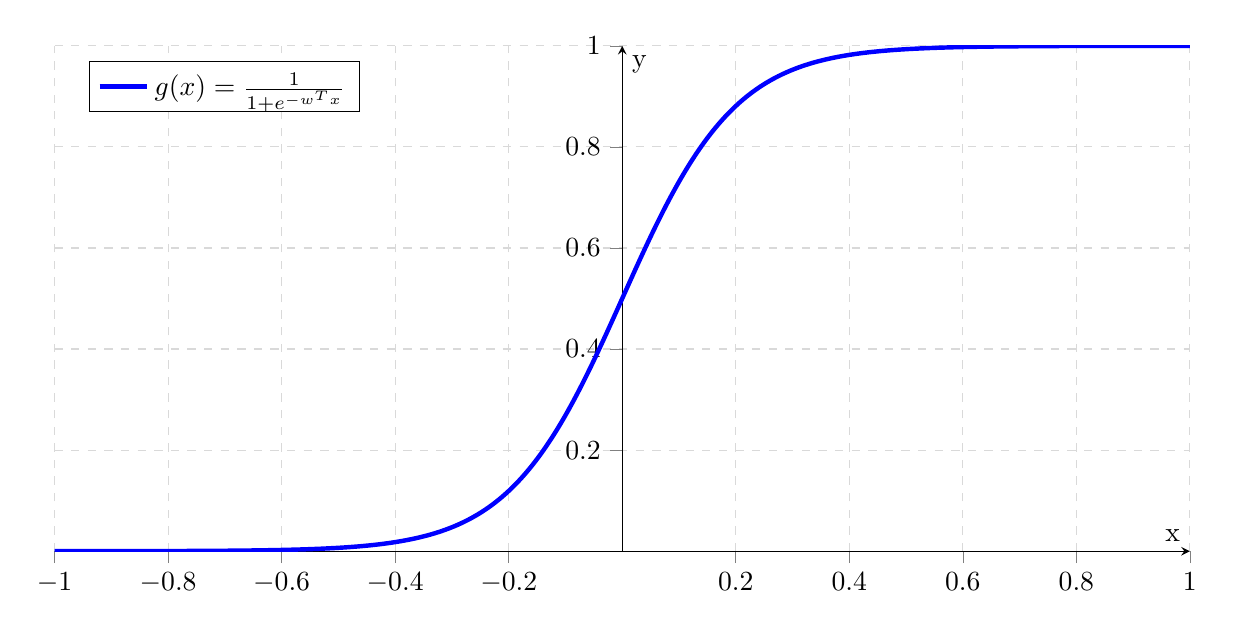
\begin{tikzpicture}
    \begin{axis}[
    	legend pos=north west,
        axis x line=middle,
        axis y line=middle,
        grid = major,
        width=16cm,
        height=8cm,
        grid style={dashed, gray!30},
        xmin=-1,     % start the diagram at this x-coordinate
        xmax= 1,    % end   the diagram at this x-coordinate
        ymin= 0,     % start the diagram at this y-coordinate
        ymax= 1,   % end   the diagram at this y-coordinate
        %axis background/.style={fill=white},
        xlabel=x,
        ylabel=y,
        tick align=outside,
        enlargelimits=false]
      % plot the stirling-formulae
      \addplot[domain=-1:1, blue, ultra thick,samples=500] {1/(1+exp(-10*x))}; 
      \addlegendentry{$g(x)=\frac{1}{1+e^{-w^Tx}}$}
    \end{axis} 
\end{tikzpicture}
\end{figure}\\*\\*
\newpage
\noindent
$\emph{Maximum Likelihood Estimate (MLE)}$ : The Logistic Regression algorithm learns weights so that it can maximise the likelihood of the data. For more detailed explanation please refer to \cite{15}. 
$$L(\vec w) = \sum_{i=1}^{n}\log g(y_iz_i),$$ 
Where $z_i = \sideset{}{_k}\sum w_kx_{ik}$. Note : $1 - g(x) = g(-x)$\\*
The MLE in sklearn\footnote{\url{http://scikit-learn.org}} uses a regularisation parameter. Hence 
$$L = - \sum_{i=1}^{n}\log g(y_iz_i) + \frac{C}{2}\sum_{k=1}^{l} w_k^2$$

\subsection{Application}
The details of the experiment are explained in the next chapter, however here we briefly address some of the points. We first split the data into training and test data sets and then transform the data such that the feature values are normalised. We then pass the training dataset with the features mentioned in section 5.1 into our Logistic Regression model. Once we train this data we then pass the test data into the model to classify and check the accuracy and other measures of this classification. We improve the correctness of this prediction by changing the regularisation parameter to avoid overfitting. 


\newpage
\section{Support Vector Machines}

\subsection{Background}
Support Vector Machines (SVM) is arguably one of the most popular supervised classification methods to date in Machine Learning \cite{31}. It is a linear machine model and the design is greatly influenced by vectors which are closest to the separating hyper plane. The reasons for choosing SVM was because they are effective in high dimensional spaces and use a subset of the training points in the decision function (called support vectors) so it is memory efficient \cite{31}. It is also versatile, in that different kernel functions can be specified for the decision functions. For instance we have used the `Radial Basis Function' kernel\footnote{$\exp(\frac{-\parallel x - x \parallel^2_2}{2\sigma^2})$,  where $\parallel x - x \parallel^2_2$ can be recognised as the squared euclidean distance between two feature vectors and $\sigma$ is a free parameter \cite{33}} and the Polynomial Kernel function\footnote{$K(x,y) = (x^Ty + c)^d$ where $x$ and $y$ are vectors and $c$ is a constant \cite{35}}. The disadvantage with SVM is that the probabilities are calculated using an expensive five-fold cross validation. Moreover if the features : data sample ratio is not fairly low then it may give poor performance. 
\subsection{Algorithm}
We have a two class problem, that is Trustworthy tweets and Untrustworthy tweets. We then have an input feature vector, $\vec x$ which we need to classify as belonging to the Trustworthy class or Untrustworthy Class.  We have a linear discriminant function : 
$$f(x) = w^Tx + b$$
\noindent
Depending on our feature space, this linear equation would be a straight line, plane or hyperplane for two, three or multidimensional feature spaces respectively. The $w$ is a vector which is perpendicular to the hyperplane and it represents the orientation of the hyper plane in our D-dimensional space where D is the dimensionality of the feature vector. The term `b' which is known as a bias term, represents the position of the hyper plane in the D-Dimensional space. In our problem, for every feature vector $\vec x$ we need to compute f(x) and if it falls on the positive side of the hyper plane then we have the following equation satisfied : 
\begin{gather}
f(x) = w^Tx + b > 0 \implies x \in \textup{Trustworthy}
\end{gather}
If it falls on the negative side of the hyper plane we have 
\begin{gather}
f(x) = w^Tx + b < 0 \implies x \in \textup{UnTrustworthy}
\end{gather}
If it falls on the plane we have this : 
\begin{gather}
f(x) = w^Tx + b = 0
\end{gather}
We need to find the $w$ and $b$ such that these values can be used in $f(x)$ to find the separating hyperplane. Hence we train such that for every training sample which belongs to the class `Trustworthy' we start with an initial value for $w$ and $b$ and we check if $f(x)$ is actually greater than 0. If it is not greater than 0 we adjust $w$ and $b$ such that the orientation and position of the hyperplane is shifted till a point where the data point is classified on the positive side of the hyper plane. Likewise we work out a similar procedure for `Untrustworthy tweets'. Let us look at the simple graph below : \\*

\begin{filecontents*}{SVMPlot.csv}
x,y,label
2,2,a
1,4,a
4,3,a
6,5,b
8,7,b
7,9,b
\end{filecontents*}
\begin{tikzpicture}
\begin{axis}
 legend pos=center,
        axis x line=middle,
        axis y line=middle,
        grid = major,
        width=16cm,
        height=6cm,
\addplot [
        % clickable coords={\thisrow{label}},
        scatter/classes={
            a={mark=square*,green},%
            b={mark=square*,red},%
            c={mark=o,draw=black,fill=black}%
        },
        scatter,only marks,
        scatter src=explicit symbolic]
	table [x=x,y=y,meta=label, col sep=comma]
            {SVMPlot.csv};
    \legend{Trustworthy,Untrustworthy}
\end{axis}
\end{tikzpicture}
\begin{gather}
w.x + \frac{b}{\parallel w \parallel} = d
\end{gather}

\noindent
Support vectors are the vectors that are closest to the hyperplane. So in the diagram above every vector that has a distance $d_{min}$ from the hyperplane is a support vector. Our goal in SVM for the hyperplane is to make sure the margin between the data points and the separating planes are as large as possible. Since generally if the margin is larger the generalisation error of the classifier will be lower. If we look at equation(5.12) we would want to maximise $d$ and this can be achieved by minimising $\mid w \mid$ and maximising bias $b$. 
In order to understand which combinations of $w$'s to use to arrive at the best possible margin we need to maximise the margin ($\frac {1}{\parallel w \parallel}$) subject to the fact that for the nearest point which would have the smallest value of $\mid w^Tx_n + b \mid$ = 1. We scale the value of $w$ to make the equation 1. To optimise this we use Lagrange multipliers\footnote{Find the min or max extremes of a function which also contains constraints \cite{32}} with KKT\footnote{Karush-Kuhn-Tucker Conditions \cite{32}} conditions for our constraints; Refer \cite{32} for more information on KKT conditions. 

\newpage
\section{Random Forests}
\subsection{Background}
Decision Tree Learning uses decision trees as a predictive model which maps observations about an item to conclusions about the items target value \cite{42}. These Decision Trees are easily understood by humans, very compact and handles missing and categorical data very well and can handle large non-linear boundaries between groups. However despite all these advantages of trees, we may not find the best tree and there are times when they are not as accurate as SVMs and other state of the art predictors. The solution for this was to use a collection of trees and is termed Random Forests.\\*\\* 
Random Forest is used for prediction, of categorical and continuous data. This method is based on Trees and is fairly simplistic, yet one of the more powerful Machine Learning models. We can see this from the performance of Random Forests in figure 5.1, where Random Forests ranks seconded topped only by Boosted Decision Trees. Random Forests (Breiman, 2001) work as a huge collection of non-correlated decision trees and it is a technique based on bagging.\footnote{Bagging or bootstrap aggregation is a technique for reducing the variance of an estimated prediction function \cite{30}}
\subsection{Algorithm}
\begin{algorithm}[h!]
  \caption{Random Forests, adapted from Trevor et al. \cite{3}}
  \begin{algorithmic}[1]
  \State Observed Data Points D = [($x_i$,$y_i$),$\hdots$,($x_n$,$y_n$)]. 
  \For{i=1 to B}\Comment{B is some number of trees}
  \State (i)Chose a bootstrap sample from $D$, called $D_i$ of size N from the 
  \State  training data.
  \State (ii)Using $D_i$ we construct a Random Forest Tree $T_i$, by re-cursively repeating
  \State  the following steps for each terminal node of the tree, until a minimum node 
  \State  size $n_{min}$ is achieved.
  \While{MinNode != $n_{min}$}
  \State At each node, chose a random subset $m$ of features from the $p$ variables
  \State (We only consider splitting on those features)
  \State Select the best variable/split-point among the m
  \State Split the node into two daughter nodes
  \EndWhile
   \EndFor
   \State We output the collection of trees $\{T_b\}_1^B$
  \end{algorithmic}
\end{algorithm}
Classification: Let $C_b(x)$ be the class prediction of the $b^th$ random-forest
tree. Then $C_{rf}^B(x)$ = majority vote $\{C_b(x)\}^B_1$.

\subsection{Application}
Below we have a Matrix of training samples with their classifiers. \\*\\*
$\textup{Data Set }= \begin{bmatrix}
\textup{ FrequencyOfTweets} & \textup{FavouriteCount} & \textup{RetweetCount} \\
12 & 4 & 6  \\
2 & 0  & 1 \\
\vdots & \vdots & \vdots \\
1 & 2 & 6  \\
5 & 7  & 10
\end{bmatrix}$
$\begin{bmatrix}
\textup{Classifier } \\
\textup{TrustWorthy } \\
\textup{UntrustWorthy} \\
\vdots \\
\textup{UntrustWorthy} \\
\textup{TrustWorthy } 
\end{bmatrix}$\\*\\*
From the above sample set and we create many random combinations of sub sets with randomly picked values from the above main set. For Eg., \\*

$\textup{Data Set 1 }= \begin{bmatrix}
12 & 4 & 6  \\
22 & 10  & 11 \\
\vdots & \vdots & \vdots \\
1 & 2 & 6  \\
15 & 27  & 10
\end{bmatrix}$
$\begin{bmatrix}
\textup{1} \\
\textup{1} \\
\vdots \\
\textup{0} \\
\textup{1} 
\end{bmatrix} \Longrightarrow \textup{Decision Tree 1} $ \\*
$\textup{Data Set 2 }= \begin{bmatrix}
14 & 14 & 6  \\
2 & 0  & 11 \\
\vdots & \vdots & \vdots \\
11 & 0 & 6  \\
5 & 7  & 1
\end{bmatrix}$
$\begin{bmatrix}
\textup{0} \\
\textup{1} \\
\vdots \\
\textup{0} \\
\textup{0} 
\end{bmatrix}  \Longrightarrow \textup{Decision Tree 2}$
\\*\\*\\*
$\textup{Data Set N }= \begin{bmatrix}
17 & 34 & 6  \\
2 & 1  & 1 \\
\vdots & \vdots & \vdots \\
1 & 2 & 6  \\
15 & 7  & 10
\end{bmatrix}$
$\begin{bmatrix}
\textup{1} \\
\textup{0} \\
\vdots \\
\textup{0} \\
\textup{1} 
\end{bmatrix}  \Longrightarrow \textup{Decision Tree N}$
\\*\\*
We now have many decision trees, each with different variations of the classifications and we use all these decision trees to create a ranking of classifiers. For Classification, each tree would provide a class vote and the final classification is based on majority vote. 
\newpage













































\chapter{Evaluation and Discussion}

In this chapter we explain our experiment and present the results obtained from our models for the problem of finding Trustworthy and Untrustworthy content on Twitter. We then discuss and generally reflect on the results obtained.

\section{Experiment}
In this section we detail our experiment and data statistics. The table below gives an overview of the variety of our data. 
\begin{center}
\captionof{table}{Data Statistics} 
\begin{tabular}{|l|l|}
\hline
Total Number of Tweets  &  17203  \\ \hline
Total Number of Unique Users & 45  \\ \hline
Number of Trustworthy Users  & 20 \\ \hline
Number of Untrustworthy Users & 25  \\ \hline
Number of Retweets   & 15364  \\ \hline
Number of non-Retweets & 2839  \\ \hline
Tweets with No Emotion &  16932\\ \hline
Happy Tweets   & 139 \\ \hline
Sad Tweets    & 132 \\ \hline
Tweets that are Replies & 381 \\ \hline
Tweets that are not replies & 16278 \\ \hline
 Features : DataPoints & 29 : 17203  \\ \hline
\end{tabular}
\end{center}
As with any Machine Learning problem, our training and testing cycle utilises a trial and error approach. This consists of training multiple data sets with data points being collected at varying points in time. The aim of this approach is to increase the performance of models on each subsequent iteration. For this task we used 80\% of the data to train the three different classifiers separately and used the remaining 20\% of the data to test the performance of our models. We also independently evaluated the results, using a raw data set which was not related to the previous dataset. That is, it consisted entirely of new tweets from new users. We hand picked some known fake tweets, particularly ones that arise during crisis situations (Tweets that have been repeatedly reported in news paper articles and other research papers) as our Untrustworthy tweets and some tweets from other news agencies for our Trustworthy tweets. This dataset consisted of 39 tweets, 20 being Untrustworthy and 19 being Trustworthy. However, we also wanted to test our model on general tweets by the average user, so we evaluated the performance of the model on a much smaller dataset of 12 tweets of which all of them but one were Trustworthy. In the next paragraph we go into detail about the parameters used in our Machine Learning models.\\*\\*
For our Logistic Regression (LR) classifier we used an L2 regularisation parameter, which is essentially a parameter that we pass into our model, which reduces overfitting $LR(L_2)$. In the case of Support Vector Machines (SVM) as mentioned in Chapter 5, we used a Radial Basis Function (\textit{rbf}) kernel. We also tried using Linear and Polynomial kernels however the best performance was achieved with \textit{rbf}. For SVM, there are two important parameters that needs to be specified. They are $C$ and $gamma$. The parameter $C$ trades off misclassification of training data against a simple decision surface [39]. $C$, when low would give a smooth decision surface, whereas when high it aims to classify all training samples correctly thereby not producing a smooth decision surface. The gamma value determines the level of influence of a single training sample. If the $gamma$ is large, then the samples should be closer to each other to be affected \cite{39}. We used 1 for $C$ and 0 for $gamma$. It is usually a good idea to change these values around to get a better decision surface. \\*\\*
In the case of the Random Forests (RF) classifier, we had to specify the number of trees we want in our model; in our case we specified 500. This is because the number of trees, is not a tuning parameter in RF. Although a high number of trees is usually always better, once we have enough trees to work with the accuracy doesn't improve, hence it would be computationally wasteful to specify more than the necessary number of trees. However in our case we used 500 as this gave us quality predictions. We used information gain\footnote{Calculates how much information we gained by doing the slicing on this particular node or feature}as the quality of our split since the gini index\footnote{The attribute value that provides the smallest split is chosen as the node to split on} gave us slightly poor performance. 
\section{Results}
In this section we present the results obtained from the three different classifiers used in our experiment above. In the following subsections we discuss accuracy, precision, recall and Area Under Curve (AUC) all of which are measurements used to measure the ability of the model to predict appropriately. 
\subsection{Accuracy, Precision and Recall}
In order to understand this section, the reader needs a clear idea of what some of the metrics we calculated represent. The table given below addresses that.\\*\\*
\begin{minipage}{\linewidth}
\centering
\captionof{table}{Measurements}
\begin{tabular}[t]{|C{.90in}|C{3.00in}|C{1.60in}|}
\toprule[1.5pt]
Measure & Explanation & Formula\\\midrule
True Positive & Correctly classified as Trustworthy - Trustworthy Tweet & TP \\
\hline
False Positive & Incorrectly classified as Trustworthy - Untrustworthy Tweet & FP \\
\hline   
True Negative & Correctly classified as Untrustworthy - Untrustworthy Tweet & TN\\
\hline
False Negative & Incorrectly classified as Untrustworthy - Trustworthy Tweet & FN\\
\hline
TPR & True Positive Rate & $\frac {TP}{TP + FN}$\\
\hline 
FPR & False Positive Rate &  $\frac {FP}{FP + TN}$\\
\hline
TNR & True Negative Rate &  $\frac {TN}{FP + TN}$\\
\hline
FNR & False Negative Rate & $\frac {FN}{TP + FN}$\\
\hline
Accuracy & The degree of closeness of measurements to the actual value &  $\frac {TP + TN}{TP + FP + FN + TN}$  \\    
\hline
Precision & The precision is the fraction of the retrieved values which are relevant  &  $\frac{TP}{TP + FP}$\\
\hline
Recall &  The recall is the fraction of relevant instances received &  $\frac{TP}{TP+FN}$\\
\hline
$F_\beta$ & This is the harmonic mean of precision and recall. We used the value `1' for $\beta$ & $(1 + \beta^2)\frac{Precision \times Recall}{\beta^2 Precision + Recall}$\\
\hline      
Support & The number of occurrences of each classification label in in truth & - \\
\hline                                                                                                                                                                                    
\bottomrule[1.25pt]
\end{tabular}
\label{tab:LPer}
\end{minipage}
\newpage
\noindent
The following table gives us the accuracy scores of each of the classifiers. As we can see from the table, RF seems to have been performing quite well on Training, Test and the new Data Set however, has performed slightly poorly in comparison to the other techniques when it tested with some random tweets from the average user. Logistic Regression, has performed quite well on all four data sets. The problem with the accuracy score is that the two different outcomes (Trustworthy and Untrustworthy) are not necessarily equal in weight. For example, if our classifier predicted that a tweet is Untrustworthy but it is, in actuality Trustworthy then this would not be much of an issue. However, if our classifier predicted an Untrustworthy tweet as Trustworthy then this might be a problem, since this is exactly how rumours spread.  \\*\\*
\begin{minipage}{\linewidth}
\centering
\captionof{table}{Accuracy} \label{tab:title} 
\begin{tabular}[t]{ C{1.4in} *3{C{1.4in}}}\toprule[1.5pt]
\bf Data & \bf Logistic Regression & \bf Support Vector Machines & \bf Random Forests \\\midrule
Training        &  0.99651  & 1.0 & 1.0\\
Test        &  0.99709     & 0.90380 & 1.0 \\
New Data        &  0.87179   & 0.48717  & 0.97435 \\
Random New Data & 0.83333 & 0.91666 & 0.41666 \\ 
\bottomrule[1.25pt]
\end {tabular}\par
\bigskip
\end{minipage}\\*\\*
\noindent
For precisely the reasons mentioned above we will look at further ways of measuring the quality of our model. Figures 6.1, 6.2 and 6.3 below, show a confusion matrix. A confusion matrix is a nice way of visualising the predictions of a classifier. The $x-axis$ represents the true values of the data points and the $y-axis$ represents the predictions made by the classifiers. We show the confusion matrix for the training data in the diagrams below, however the matrix of the new dataset and the random new dataset can be found in the appendix. In this matrix data points belonging to coordinates $(0,0) , (1,1)$ are correctly classified and points that fall in the $(0,1) , (1,0)$ box are incorrectly classified. One way to look at this matrix would be,\textit{ `When a tweet is Trustworthy, how often do our models classify this correctly?'}. A measure such as this is called `Recall' and by looking at the three diagrams below we can see that SVM and Random Forests have a high recall score (They predict 2293 times correctly out of the total of 2293). The other question we could ask to understand this diagram is \textit{`When our model predicts that a tweet is Trustworthy, how often is it actually Trustworthy?'}. This is known as the precision. Looking at our diagrams we could say that Random Forests give us the best score here as it correctly predicts 2293 out of 2293 instances, where as the LR and SVM fall behind by 2292 out of 2299 and 2293 out of 2624 respectively. In tables 6.4 and 6.5 we show the precision and recall measures for our different datasets.   \\*\\*

\begin{minipage}{\linewidth}
\centering
\captionof{table}{Precision} \label{tab:title} 
\begin{tabular}[t]{ C{1.4in} *3{C{1.4in}}}\toprule[1.5pt]
\bf Data & \bf Logistic Regression & \bf Support Vector Machines & \bf Random Forests \\\midrule
Training        &  0.99528  & 1.0 & 1.0\\
Test        &  0.99608     & 0.87385 & 1.0 \\
New Data        &  0.84999   & 0.48717  & 0.95000 \\
Random New Data & 1.0 & 0.91666 & 1.0 \\ 
\bottomrule[1.25pt]
\end {tabular}\par
\bigskip
\end{minipage}\\*\\*

\begin{minipage}{\linewidth}
\centering
\captionof{table}{Recall} \label{tab:title} 
\begin{tabular}[t]{ C{1.4in} *3{C{1.4in}}}\toprule[1.5pt]
\bf Data & \bf Logistic Regression & \bf Support Vector Machines & \bf Random Forests \\\midrule
Training        & 0.99956  & 1.0 & 1.0\\
Test        &  0.99956     & 1.0 & 1.0 \\
New Data        &  0.89473  & 1.0  & 1.0 \\
Random New Data & 0.90000 & 1.0 & 0.36363 \\ 
\bottomrule[1.25pt]
\end {tabular}\par
\bigskip
\end{minipage}\\*\\*

\begin{figure}[!h]
  \centering
\includegraphics[width=10cm]{LRCMTestData}
  \caption[Logistic Regression Confusion Matrix]
   {Logistic Regression Confusion Matrix}
\end{figure}

\begin{figure}[!h]
 \centering
\includegraphics[width=10cm]{SVMCMTestData}
  \caption[Support Vector Machine Confusion Matrix]
   {Support Vector Machine Confusion Matrix}
\end{figure}

\begin{figure}[!h]
 \centering
\includegraphics[width=10cm]{RFCMTestData}
  \caption[Random Forests Confusion Matrix]
   {Random Forests Confusion Matrix}
\end{figure}

\subsection{Probabilities}
Delving further into measuring the quality of our system, sometimes decision making can favour a probability estimation over a simple classification. In some cases it makes more sense to say `\textit{This person has a 90\% chance to pass the exam}' as opposed to saying `\textit{You will pass}'. However assessing how good a model is when we have probabilities as opposed to classifications could be quite difficult. Ergo we predict the probabilities of a tweet being Trustworthy or not then calculate the TPR and FPR and plot this on a graph. The graph below plots the TPR values on the $x-axis$ and FPR values on the $y-axis$. The top left corner of the graph is the most ideal point since it has a FP rate of 0 and a TP rate of 1. We ideally want to maximise the TPR while minimising the FPR. AUC, is the area under the curve, which essentially refers to the area within the curve created by out plot. We therefore aim to achieve a high AUC score. The table 6.6 gives the AUC scores of our classifiers and the figures 6.4,6.5 and 6.6 below demonstrate the AUC for our different datasets. \\*\\*

\begin{minipage}{\linewidth}
\centering
\captionof{table}{Area Under Curve} \label{tab:title} 
\begin{tabular}[t]{ C{1.4in} *3{C{1.4in}}}\toprule[1.5pt]
\bf Data & \bf Logistic Regression & \bf Support Vector Machines & \bf Random Forests \\\midrule
Test        &  0.99999     & 0.99742 & 1.0 \\
New Data        &  0.94342  & 0.5000  & 0.97632 \\
Random New Data & 1.0 & 0.5000 & 1.0 \\ 
\bottomrule[1.25pt]
\end {tabular}\par
\bigskip
\end{minipage}\\*\\*

\begin{figure}[!h]
 \centering
\includegraphics[width=10cm]{LRROCAUC}
  \caption[Logistic Regression AUC]
   {LR ROC Area Under Curve}
\end{figure}

\begin{figure}[!h]
 \centering
\includegraphics[width=10cm]{SVMROCAUC}
  \caption[Support Vector Machine AUC]
   {SVM ROC Area Under Curve}
\end{figure}

\begin{figure}[!h]
 \centering
\includegraphics[width=10cm]{RFROCAUC}
  \caption[Random Forests AUC]
   {RF ROC Area Under Curve}
\end{figure}\leavevmode 

\section{Discussion}
In the previous section, we presented three different ways of measuring the quality of our predictors. They are accuracy, precision and recall and AUC. As we can observe from the results above some measurements rate some classifiers as better than the others and this rating could be just the opposite for another measurement we take. We know that  measurements do not always produce a high number for a good classifier and a low number for a bad classifier.  They just present to us some information about the model and we make choices on which model best suits our problem, which would be based on scalability, reliability, precision and other such factors.\\*\\* 
From the above observations it is apparent that Random Forests gives us the best performance for this problem. It performs equally or better than the other two models at all three measurements. Features such as \textit{Emotions, Retweet/Tweet, Frequency of tweets, Tweet length and Favourites count} were considered most important by this model. \textit{In Reply to a Status ID, In Reply to a User ID,  Profile URL, Length of the user description string and User mentions} were considered least important to give us the best performance.  We found that we could accurately predict Trustworthiness to 97\% using the Random Forest Classifier. However, this level of accuracy is achieved when we use the model to determine the trustworthiness of Tweets that are either completely Trustworthy or completely Untrustworthy. This could be a classic case of over fitting where our model was designed around perfect tweets and imperfect ones. Although we had approximately 20,000 Tweets to train from, our user base was much smaller (approximately 40). This also meant that the user based features that we chose would have repeated significantly during our training. \\*\\*
To test if our model was $\textbf{overfitted}$, we collected an additional 39 data points, most of them from very different users so there was very little repetition of features pertaining to the user, and tested our models on it. As we saw from the previous section, apart from SVM, both LR and RF had reasonably good predictions. We now give an example of a tweet that both the LR and RF models predicted inaccurately and discuss the possible reasons for this. \\*\\*
\centerline{\textit{UK government exploring origami as possible solution to housing shortage: }} 
\centerline{\textit{paper house in London may cost ``as little as 450,000''}}\leavevmode \\\\
This is an Untrustworthy tweet classified as Trustworthy by both our best performing Machine Learning models. This was posted by a user account named \textit{falsenews}. In terms of the features of this user, the profile has 380 tweets to date and 108 followers and 0 friends. This is very unlike any of the Trustworthy user profiles we trained on. Having said this, the feature \textit{Default Profile}, which tells you if the profile has been changed since it was created is \textit{false} which is the case for most other news agencies. In terms of the tweet features \textit{ tweet length, number of smilies, emotion of the tweet, wrongly used keywords and retweet} this tweet closely resembles Trustworthy tweets. Considering the fact that some of the above mentioned features are weighted more, by our RF this tweet is very similar to a Trustworthy tweet, which might probably be the reason for misclassification of this tweet. \\*\\*
To check if our model could be $\textbf{generalised}$ such that it predicts accurately, tweets by the general user, which does not necessarily have strong characteristics of Trustworthy and Untrustworthy tweets as identified before by our RF classifier we collected 12 data points, 11 of which were Trustworthy. These tweets were from Twitter users who posted Trustworthy tweets and this was manually verified by us. Unfortunately our best predictor the RF classifier did not perform really well on this dataset. Of the 12 data points it predicted 5 accurately, which is a decent score. The LR classifier predicted 10 data points accurately and SVM predicted 11 points accurately. However our SVM model has a slight tendency to predict Untrustworthy tweets as Trustworthy and  Trustworthy tweets as Trustworthy hence this dataset would have been slightly biased to the advantage of our SVM classifier since we had a ratio of 11 : 1 of Trustworthy and Untrustworthy tweets. Let us look at another example. \\*\\*
\centerline{\textit{A bizarre legal loophole in New Orleans allows for drive-thru }}
\centerline{\textit{daiquiri outlets [video] http://t.co/4EQ7iI4JHX via @VICEUK}}\leavevmode \\\\
This is a Trustworthy tweet classified as Untrustworthy by both RF and LR. The user account has 37986 followers, 6675 friends a Favourites count of 3709 and a total of 7735 tweets. Although this level of propagation is not nearly as much as news agencies, this certainly is a high number for an individual user. We had two tweets from the same user, and RF predicted both the tweets as Untrustworthy which could mean that it could have given some preference to the User account information as opposed to the tweet itself. However LR predicted one as Trustworthy and this as Untrustworthy which could mean that it gave more preference to the Tweet content / Tweet features. It would be interesting to analyse these further at some point. Unfortunately, the SVM model did not perform without bias on datasets that it was not trained on hence we have omitted the classifications by SVM in our discussions.\\*\\*
 \noindent
Another significant observation from our research was that there were many profiles and characteristics of tweets that appeared legitimate but provided wrong information. For example, A user named ComfortablySmug tweeted this in the wake of hurricane Sandy\footnote{http://www.economist.com/news/united-states/21588125-recovery-has-been-remarkable-damage-persists-stronger-storm}:\\*\\*
\centerline{\textit{"BREAKING: Confirmed flooding on NYSE.}} \\* \centerline{\textit{The trading floor is flooded under more than 3 feet of water."}}\leavevmode \\\\
This user seems extremely legitimate, also has a decent amount of followers and worked in research at a hedge fund \cite{37}. One would believe that a user of such high calibre would not spread false information. In fact tweets from reputable users such as this would still be hard to identify using our model, since the user contains all the necessary characteristics of a Trustworthy person. Apart from the person, the tweet was also widely spread, favourited and retweeted many times. These are some other characteristics of Trustworthy tweets, hence making the task of distinguishing between popular and Trustworthy tweets become increasingly hard. \\*\\*
Having said this, our model does predict to some level, tweets that don't fall strongly into either of the above category (Trustworthy / Untrustworthy). We have seen this from the example data set we tested our models from. However, this is not to this great level of accuracy. On the other hand, our aim was to classify tweets as Trustworthy or Untrustworthy if they were. The purpose was to be able to use this analysis in crisis situations or in circumstances where this differentiation can be important. For example; 
\begin{figure}[h!]
  \centering
\includegraphics[width=10cm]{Ted}
  \caption[Unimportant Tweet]
   {Unimportant Tweet}
\end{figure}\leavevmode\\*
For a tweet such as the one above, we have no reason to provide Trustworthiness metrics or classification as the tweet serves no useful purpose and is purely someones opinion which does not affect anyone else personally or otherwise. \\*\\*
\noindent
We chose features from three different categories. We had $\textup{Message\_Based}$ Features, $\textup{User\_Based}$ Features and $\textup{Tweet\_Based}$ Features. In terms of $\textup{Message\_Based}$ Features, we initially only had \textit{tweet length, presence of URL, media type} and such generic details obtained from the Twitter API. The accuracy of predicting with purely the above features was slightly lower than the final accuracy we achieved. As can be seen our most successful model did perform well when it gave importance to features such as \textit{Emotions, Tweeting frequency} etc. However, now we have included and tested features like the emotion portrayed by the tweet (e.g, Happy, Sad, NoEmotion), the number of emoticons in the tweet and also, checks for keywords like `SHOCKING', `UNBELIEVABLE' etc. We observed that words of this nature were only used by accounts that were trying to gain the user attention, and truly Trustworthy profiles do not use such words to propagate information. We noticed slight improvements in prediction, with the incorporation of such detail. \\*\\*
Interestingly the accuracy of the prediction for the new data significantly increased when we filtered the training and testing datasets to either Happy or Sad tweets. This could be due to several reasons, one of which could be that if a tweet shows emotion in terms of smilies, then it has a higher tendency to be Untrustworthy than a tweet without smilies. This was one of the characteristics that we observed from the data that we gathered and has also been observed by Aditi Gupta et al. in \cite{11}. Hence training purely on tweets with emoticons we know that any of those tweets are Untrustworthy, hence predicting the rest as Trustworthy. This could also be due to the fact that a fair number of tweets with emoticons also consisted some of the reserved words such as `LEAKED', `REVEALED' etc. \\*\\*
We used several $\textup{User\_Based}$ features for our training however as mentioned earlier, the fact that we had only 45 listed users, and approximately 20,000 tweets from all of them. This meant constant repetition of user information throughout the training of data. We used the \textit{user location} as one of the parameters in our analysis however later realised that this does not produce accurate predictions. This may be due to the fact that we had a very small sample set of users from different countries.  So this would mean that if there was one profile from the Russia in our dataset and we had classified this profile as Untrustworthy then every other profile from Russia would also be graded slightly similarly depending on the weight given for location. We decided to drop this feature until we possessed a much larger user base to analyse. We thought that the \textit{length of the description string} for each user would be a good indication of how Trustworthy the profile is, however this was deemed unimportant by our Random Forest Classifier. We also noticed that the number of friends news profiles had was significantly lower than the number of people who followed these profiles. This was originally a concern as this could bias our analysis very much, however as we normalised the dataset this was not much of a problem. \\*\\* 
\noindent 
Below we suggest some future improvements to this model. We could further delve deeper and check the media associated to the message content, by verifying the validity of the URLs, Videos and Photos presented to us. For example, During the time when a Malaysian Airline MH370 initially went missing earlier this year, there were quite a few videos of the plane being found in some ocean or on land. One such example where a non working URL directing to a blank page, in the figure below:\\*\\*
\begin{figure}[hb]
  \centering
\includegraphics[width=10cm]{MalaysianAIrlines}
  \caption[MH370]
   {Malaysian Airlines Found in Southern Indian Ocean}
\end{figure}\leavevmode\\
\noindent
When clicking this URL, there appears to be no page linked to this. The user is also not the real CNN. In terms of videos posted, we could first check if a video exists at the location specified and secondly check the source of the video. We could also provide trust scores for some of the popular video streaming services such as YouTube, Vevo, YouView\footnote{\url{http://www.techradar.com/news/television/16-best-tv-streaming-services-1044010}} or news channels as opposed to an unknown website from which the video is available. Again this was apparent during the MH370 crisis where there were videos posted of planes in different oceans, most of which were either fake videos or non-existent links to videos.  Some other interesting features to measure in Message Content would be the amount of exclamation marks used, capitalisation and other special characters used. We could also go as far as analysing the profiles / trustworthiness scores of people that the current user has either mentioned or replied to in a message and factor that into our training. \\*\\*
\noindent
It would be interesting to perform some content based analysis for descriptions of user profiles as well as the names of the users, looking at key words and phrases. For example if we had checked the credibility of the name of the user for the tweet by \textit{falsenews} discussed above, we might have been able to avoid such classification mistakes. 
\section{Summary}
In this chapter we have highlighted the experiment conducted to assess the Trustworthiness metrics of Twitter. We have shown that the Random Forests Classifier worked best for most Tweets, but the Logistic Regression classifier provided a more generalised solution, in that its' ability to predict accurately tweets from general users. We have achieved 87\% and 97\% accuracies by Logistic Regression and Random Forests respectively. We have stated the most important features used in this analysis and provided examples to explain this further.  Our aim, was to learn features from known News Websites and known Untrustworthy websites and design a model that will predict a classifications which were accurate  at least 80\% of the time. From the discussion above, we have proved that our aim was met. In the next chapter we discuss some future improvements to the system and suggest a different approach to the problem as well as provide a conclusion.  
\chapter{Reflection}
\section{Conclusion}
It takes only a few seconds to post something on Twitter. It takes even less time, to retweet a news feed on Twitter. If thousands of people take to retweeting a piece of information news can go viral within minutes. The problem arises when a piece of information spread, is not trustworthy and is false information. This could harm a lot of people concerned, particularly if this is a crisis situation. Hence Trust Metrics is an important measure to have in social media, for a more reliable online experience.\\*\\*
In this dissertation, we considered one method to differentiate Trustworthy information from Untrustworthy information. We focused on the Twitter platform, and assumed that news tweets are Trustworthy, and learned characteristics from these news tweets and used this learning to predict if other tweets are Trustworthy or not. Likewise we learned the characteristics of Untrustworthy tweets from fake twitter profiles that post Untrustworthy information and similarly used this learning to predict if other tweets are Untrustworthy or not. \\*\\*
The aim of our project was to attain at least an 80\% accuracy rate, in predicting if tweets were Trustworthy or not. In order to achieve this we used three different Machine Learning Techniques, namely Logistic Regression, Support Vector Machines and Random Forests. Using these and a collected set of data of Trustworthy and Untrustworthy tweets, we trained and tested the model such that we gain the maximum accuracy rate as possible. We have shown the Random Forests and Logistic Regressions predict with an accuracy of over 85\%. \\*\\*
We can see from our results that we have have achieved our aim. We can conclude by saying that learning Trust features from News Tweets and Fake Twitter profiles is a reliable way of learning the different characteristics of Trustworthy and Untrustworthy tweets. 
\section{FutureWork}
Future work could include extending on the current model or taking a new approach to solving this problem and later comparing it with the current predictions we have. When it comes to extending the current model, I believe that there are quite a few features that we may be able to add to the current feature set. This may or may not improve accuracy or generalise the model but we could test with different features to check how the model performs. For instance as mentioned in the previous chapter we could perform more tweet content based analysis. We could analyse the twitter feeds in verifying any external links, videos or photos posted as well as words used, calibre of words used, the grammar punctuation etc.  Again as suggested earlier we could include third party analysis, i.e give a rating to someones followers, people they respond to, people they constantly tweet to or receive tweets from and use this to train the data as well. \\*\\*
I would also like to suggest a different approach to the problem of Trust Metrics. In this, we focus on current affairs or trending topics and gather all the tweets that are tweeted regarding the topic. (This could possibly be a hashtag or the trending hashtags). We also have a listed collection of News Websites from all over the world. In this method we check Trustworthiness purely based on the content of the message as opposed to other features. We would then check if the content that is posted on some Twitter users' profile is similar to or different to what the Trusted media would be tweeting about. For example if a statement like "The London bridge is on Fire" was posted by some person and we have another tweet by BBC mentioning that "The London bridge is NOT on fire" then we would classify the former tweet as Untrustworthy. It would be interesting to compare results we received using this method and the method we devised in this dissertation.
\include{bibliography}

%now enable appendix numbering format and include any appendices
\appendix
\include{appendix1}

%next line adds the Bibliography to the contents page
\addcontentsline{toc}{chapter}{Bibliography}
%uncomment next line to change bibliography name to references
%\renewcommand{\bibname}{References}
\bibliography{bibliography}        %use a bibtex bibliography file refs.bib
\bibliographystyle{plain}  %use the plain bibliography style

\end{document}
